\documentclass[twocolumn,prd,aps,superscriptaddress,preprintnumbers,tightenlines,showpacs,nofootinbib,eqsecnum,amsfonts,amsmath,longbibliography]{revtex4-2}
\usepackage{epsfig}
\usepackage{graphics}
\usepackage{graphicx}
\usepackage[dvipsnames]{xcolor}
\usepackage{bm}
% \usepackage{txfonts}
\usepackage{amssymb}
\usepackage{xspace}
\usepackage[normalem]{ulem} % To get strikethrough (\sout)
\usepackage[colorlinks]{hyperref}
\usepackage[caption=false]{subfig}
\usepackage{booktabs}
\usepackage{url}
\usepackage{float}
\usepackage[bottom]{footmisc}
\usepackage{lineno}
\usepackage{mathrsfs}
\usepackage{makecell}
\usepackage{microtype}

\usepackage{tikz}

\definecolor{LinkColor}{rgb}{0.75, 0, 0}
\definecolor{CiteColor}{rgb}{0, 0.5, 0.5}
\definecolor{UrlColor}{rgb}{0, 0, 0.75}
\definecolor{rred}{RGB}{218,41,28}
\hypersetup{linkcolor=NavyBlue}
\hypersetup{citecolor=NavyBlue}
\hypersetup{urlcolor=NavyBlue}

\usepackage{perpage}
\MakePerPage{footnote}

\newcommand{\paperone}{Paper~I\xspace}

\newcommand{\h}{\mathpzc{h}}
\newcommand{\Hhat}{\hat{\mathpzc{H}}}
\newcommand{\B}{\mathpzc{B}}
\newcommand{\hlm}{\mathpzc{h}_{\ell m}}
\newcommand{\xilm}{\xi_{\ell m}}
\newcommand{\Ylm}{{Y}^{-2}_{\ell m}}
\newcommand{\Y}{{Y}^{-2}}
\newcommand{\hc}{h_\times}
\newcommand{\hp}{h_+}
\newcommand{\Fc}{F_\times}
\newcommand{\Fp}{F_+}
\newcommand{\Mf}{M_f}
\newcommand{\cA}{\mathpzc{A}}
\newcommand{\lm}{_{\ell m}}
\newcommand{\deff}{d_\mathrm{eff}}
\newcommand{\rmi}{\mathrm{i}}
\newcommand{\blambda}{\bm{\lambda}}
\newcommand{\btheta}{\bm{\theta}}
\newcommand{\bxi}{\bm{\xi}}
\newcommand{\bxigr}{\bm{\xi}_{\text{GR}}}
\newcommand{\bxingr}{\bm{\xi}_{\text{nGR}}}
\newcommand{\bzeta}{\bm{\zeta}}
\newcommand{\bs}[1]{\bm{\vec{S}_{#1}}}
\newcommand{\Mo}{M_{\odot}}
\newcommand{\FFe}{\mathrm{FF}_\mathrm{eff}}
\newcommand{\FF}{\mathrm{FF}}
\newcommand{\e}{\mathrm{e}}
\newcommand{\rhoopt}{\rho_\mathrm{opt}}
\newcommand{\rhosubopt}{\rho_\mathrm{subopt}}
\newcommand{\fqnm}{f}
\newcommand{\sigmaqnm}{\sigma}
\newcommand{\n}{\mathbf{n}}
\newcommand*{\skymapscale}{0.5}
\newcommand*{\paramestscale}{0.455}
\newcommand{\df}[1]{\delta f_{\text{#1}}}
\newcommand{\dtau}[1]{\delta \tau_{\text{#1}}}
\newcommand{\fngr}[1]{f_{\text{#1}}}
\newcommand{\taungr}[1]{\tau_{\text{#1}}}
\newcommand{\fgr}[1]{f ^{\text{GR}}_{\text{#1}}}
\newcommand{\taugr}[1]{\tau ^{\text{GR}}_{\text{#1}}}
\newcommand{\pSEOB}{\texttt{pSEOBNR}}
\newcommand{\SEOB}{\texttt{SEOBNR}}

% Modified gravity related
\newcommand{\pd}{\partial}
\newcommand{\dd}{{\rm d}}
\newcommand{\dV}{{\rm d}^{4}x \, \sqrt{-g} \,}

\newcommand{\lame}{\lambda_{\rm e}}
\newcommand{\lamo}{\lambda_{\rm o}}
\newcommand{\acs}{\ell_{\rm CS}}
\newcommand{\agb}{\ell_{\rm GB}}

% Comment commands
\newcommand{\ag}[1]{{\textcolor{cyan}{{[AG: #1]}} }}
\newcommand{\hs}[1]{{\textcolor{blue}{{[HS: #1]}} }}
\newcommand{\ab}[1]{{\textcolor{green}{{[AB: #1]}} }}

\newcommand{\AEI}{\affiliation{Max Planck Institute for Gravitational Physics (Albert Einstein Institute), Am M\"uhlenberg 1, Potsdam 14476, Germany}}
\newcommand{\UMD}{\affiliation{Department of Physics, University of Maryland, College Park, Maryland 20742, USA}}

\begin{document}

% HS: temporary title. Feel free to add suggestions
% \title{Probing higher-curvature gravity theories from binary black hole ringdown signals}
\title{Black-hole ringdown as a probe of higher-curvature gravity theories}

\author{Hector O. Silva}
\author{Abhirup Ghosh}
\AEI
\author{Alessandra Buonanno}
\AEI
\UMD

\date{\today}


%%%%%%%%%%%%%%%%%%%%%%%
\begin{abstract}
\end{abstract}
%%%%%%%%%%%%%%%%%%%%%%%

\maketitle
% \tableofcontents

%%%%%%%%%%%%%%%%%
\section{Introduction}
\label{sec:intro}
%%%%%%%%%%%%%%%%%

\hs{AB will do this.}

%%%%%%%%%%%%%%%%%
\section{Methods}
\label{sec:method}

\subsection{The parametrized ringdown spin expansion coefficients formalism}
\label{sec:review_parspec}

\hs{HS will do this.}
\hs{Here we briefly review~\cite{Maselli:2019mjd,Carullo:2021dui}.}

The formalism modifies the Kerr quasinormal mode frequency as
%
\begin{subequations}
\begin{align}
\omega_{\iota} &= \omega^{\rm K}_{\iota} \, (1 + \delta \omega_{\iota}), \\
\tau_{\iota}   &= \tau^{\rm K}_{\iota}   \, (1 + \delta \tau_{\iota}),
\end{align}
\label{eq:general_deviation}
\end{subequations}
%
where the $\iota$ collectively represents the QNM labels $\{l,\, m,\, n\}$.


Further expand the Kerr expression as:
%
\begin{subequations}
\begin{align}
\omega_{\iota} &= (1/M) \sum_{j = 0}^{N} \, \chi^{j} \omega^{(j)}_{k} \, \left( 1 + \gamma \delta \omega^{(j)}_{k} \right), \\
\tau_{\iota}   &= M     \sum_{j = 0}^{N} \, \chi^{j} \tau^{(j)}_{k}   \, \left( 1 + \gamma \delta \tau^{(j)}_{k} \right),
\end{align}
\label{eq:kerr_expansion}
\end{subequations}

Also,
%
\begin{equation}
\gamma = \frac{\kappa}{M_{\rm s}^{p}} = \frac{\kappa (1 + z)^{p}}{M^{p}}
= \left[
\frac{\ell c^2 (1 + z)}{G M}
\right]^{p}
\end{equation}
%

\subsection{The parametrized waveform model}
\label{sec:review_pSEOB}

\hs{AG will do this.}
\hs{Here we present a short review of~\cite{Brito:2018rfr,Ghosh:2021mrv} and
explain how we modified it to include the {\sc Parspec} parametrisation.}

\subsection{Overview of modified gravity theories}
\label{sec:review_theories}

We will consider several modified gravity theories as applications of the \pSEOB{}
waveform model presented in Sec.~\ref{sec:review_pSEOB}.
%
In the following, we briefly review which theories we consider, what are the
currents observational constraints in each of them and what we known about the
QNMs of black holes in each of them.

\subsubsection{scalar-Gauss-Bonnet gravity}
%
This theory is given by the following action,
%
\begin{equation} \label{eq:action_sgb}
    S_{\rm GB} = \frac{1}{16 \pi}
    \int \dV
    \left[
    R - \tfrac{1}{2}(\nabla \varphi)^2
    + \tfrac{1}{4} \ell^{2}_{\rm GB} f(\varphi) \mathscr{G}
    \right],
\end{equation}
%
where $R$ is the Ricci scalar associated with the metric $g_{\alpha\beta}$ and
$\varphi$ is a dynamical scalar field which couples to the Gauss-Bonnet
invariant $\mathscr{G}$,
%
\begin{equation} \label{eq:def_gb}
    \mathscr{G} =
    R^{\mu\nu\rho\sigma}R_{\mu\nu\rho\sigma}
    - 4 R^{\mu\nu}R_{\mu\nu}
    + R^2,
\end{equation}
%
with strength set by the dimensionful coupling constant $\agb$ with dimensions
of length.

Different subclasses of this theory are determined by the function $f(\varphi)$
and they can be classified into two classes based on the properties of their black hole solutions.
%
In the first class, the first derivative of the coupling
function $f'(\varphi) = \dd f  / \dd \varphi$ is always nonzero and black holes
are known to always support (secondary) scalar hair.
%
Examples include the shift-symmetric $f \propto \varphi$ and dilatonic
$f \propto \exp(\varphi)$ couplings.
%
In the second class, $f'(\varphi) = 0$ can vanish for some constant $\varphi_0$.
%
In this case, one can show that theory admits the same stationary,
asymptotically flat black hole solution of GR and scalarized black
holes~\cite{Doneva:2017bvd,Silva:2017uqg,Dima:2020yac,Herdeiro:2020wei,Berti:2020kgk}.
%
Examples include the quadratic $f \propto \varphi^2$~\cite{Silva:2017uqg}
and Gaussian $f \propto \exp(-\varphi^2)$~\cite{Doneva:2017bvd} couplings.
%
Here will consider only the dilatonic theory.

Black holes in both classes support monopolar scalar hair and thus, when in binaries,
can source scalar dipole radiation and are therefore prone to be constrained with
GWs observations of compact binaries~\cite{Nair:2019iur,Perkins:2021mhb}.
%
\dots

The calculation of the QNMs in this theory is more complicated than in GR already for
nonrotating black holes. The reason is due to the coupling between scalar field and
the Gauss-Bonnet invariant, which manifests into a coupling between scalar perturbation
and gravitational perturbations of polar parity \dots

\begin{figure}
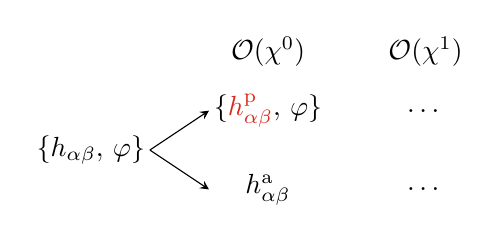
\begin{tikzpicture}[baseline,>=stealth]
    % \draw[help lines, gray] (-4, -2) grid (4, 2);
    \draw[->] (-2.5, 0) -- (-1.75, +0.5);
    \draw[->] (-2.5, 0) -- (-1.75, -0.5);

    \node at (-3.25, 0) {$\{h_{\alpha\beta}, \, \varphi\}$};

    \node at (-1, 1.25) {${\cal O}(\chi^{0})$};
    \node at (-1, +0.5) {$\{ \textcolor{rred}{h^{\rm p}_{\alpha\beta}}, \, \varphi\}$};
    \node at (-1, -0.5) {$h^{\rm a}_{\alpha\beta}$};

    \node at (+1, 1.25) {${\cal O}(\chi^{1})$};
    \node at (+1, +0.5) {\dots};
    \node at (+1, -0.5) {\dots};
\end{tikzpicture}
\caption{Quasinormal modes of black holes in scalar-Gauss-Bonnet gravity.}
\end{figure}

\subsubsection{dynamical Chern-Simons}

This theory is given by the following action,
%
\begin{equation} \label{eq:action_dcs}
    S_{\rm CS} = \frac{1}{16 \pi}
    \int \dV
    \left[
    R - \tfrac{1}{2}(\nabla \vartheta)^2
    + \tfrac{1}{4} \ell^{2}_{\rm CS} \, \vartheta \, {}^{*}RR
    \right],
\end{equation}
%
where $\vartheta$ is a pseudo-scalar field, which couples
to the Pontryagin density,
%
\begin{equation}
    {}^{*}RR = {}^{*}R^{\mu}{}_{\nu}{}^{\rho\sigma} R^{\nu}_{\mu\rho\sigma},
\end{equation}
%
where ${}^{*}R^{\mu}{}_{\nu}{}^{\rho\sigma}$ is the dual of the Riemann tensor,
defined as
%
${}^{*}R^{\mu}{}_{\nu}{}^{\rho\sigma} =
\tfrac{1}{2} \epsilon^{\mu}{}_{\nu\gamma\delta}
R^{\gamma\delta\rho\sigma}$,
%
and where $\epsilon^{\mu}{}_{\nu\gamma\delta}$ is the Levi-Civita tensor.
%
The coupling between scalar field and the Pontryagin density is set by the
$\ell_{\rm CS}$ with dimensions of length.

The theory admits the Schwarzschild black hole solution of GR, but predicts
that spinning black holes have (secondary) scalar hair, which, unlike in
scalar-Gauss-Bonnet gravity, is dipolar~\cite{Yunes:2009hc,Konno:2009kg}.
%
Consequently, the leading-scalar radiation channel is quadrupolar making this
theory presently unconstrained by from the GWs from the inspiral of black hole
binaries alone~\cite{Nair:2019iur,Perkins:2021mhb}.
%
However, the theory has been constrained by Ref~\cite{Silva:2020acr} through a
combination information of x-ray observations of the isolated neutron star PSR
J0030+0451~\cite{Lommen:2000yt,NANOGrav:2017wvv} by the
NICER~\cite{Riley:2019yda,Miller:2019cac} and gravitational-wave observation of
the binary neutron star event GW170817~\cite{TheLIGOScientific:2017qsa}.

Similarly to the case of scalar-Gauss-Bonnet gravity, the perturbations of nonrotating
black holes in dynamical Chern-Simons gravity also have a coupling between scalar and
metric perturbations. However, the coupling is between the scalar and gravitational perturbations
of axial parity~\cite{Yunes:2007ss,Cardoso:2009pk,Molina:2010fb,Wagle:2021tam}.

\begin{figure}
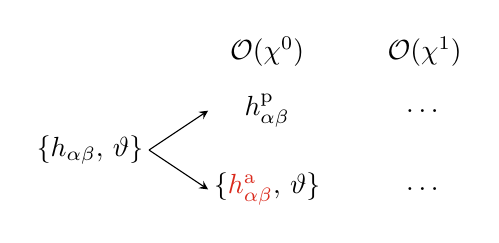
\begin{tikzpicture}[baseline,>=stealth]
    % \draw[help lines, gray] (-4, -2) grid (4, 2);
    \draw[->] (-2.5, 0) -- (-1.75, +0.5);
    \draw[->] (-2.5, 0) -- (-1.75, -0.5);

    \node at (-3.25, 0) {$\{h_{\alpha\beta}, \, \vartheta\}$};

    \node at (-1, 1.25) {${\cal O}(\chi^{0})$};
    \node at (-1, +0.5) {$h^{\rm p}_{\alpha\beta}$};
    \node at (-1, -0.5) {$\{ \textcolor{rred}{h^{\rm a}_{\alpha\beta}}, \, \vartheta\}$};

    \node at (+1, 1.25) {${\cal O}(\chi^{1})$};
    \node at (+1, +0.5) {\dots};
    \node at (+1, -0.5) {\dots};
\end{tikzpicture}
\caption{Quasinormal modes of black holes in dynamical Chern-Simons gravity.}
\end{figure}

\subsubsection{Effective-field-theory of GR}

This theory is given by the following action,
%
\begin{equation} \label{eq:action_eft}
    S_{\rm EFT} = \frac{1}{16 \pi}
    \int \dd^4x \sqrt{-g}
    \left[ R
    +
    \footnotesize{\sum}_{n \geqslant 2} \ell^{2n - 2} L^{(2n)}
    \right],
\end{equation}
%
where $\ell$ is some length scale, assumed to be small compares to the length
scale associated with a black hole, i.e., $\ell / M \ll 1$, and
$L^{(2n)}$ are corrections to the Einstein-Hilbert term action that
introduce involving higher-order curvature tensors (with $2n$ metric
derivatives).

More specifically, we follow Refs.~\cite{Cano:2020cao,Cano:2021myl} and work up
to dimension-eight operators (i.e., $n=4$),
%
\begin{subequations}
\label{eq:action_mods}
\begin{align}
    L^{(6)} &= \lame R_{\mu\nu}{}^{\rho\sigma} R_{\rho\sigma}{}^{\gamma\delta} R_{\gamma \delta}{}^{\mu\nu}
    \nonumber \\
            &\quad + \lamo R_{\mu\nu}{}^{\rho\sigma} R_{\rho\sigma}{}^{\gamma\delta} \tilde{R}_{\gamma \delta}{}^{\mu\nu},
    \label{eq:s_6}
    \\
    L^{(8)} &= \varepsilon_{1} \mathcal{C}^2
    + \varepsilon_{2} \tilde{\mathcal{C}}^{2}
    + \varepsilon_{3} \mathcal{C} \tilde{\mathcal{C}},
\label{eq:s_8}
\end{align}
\end{subequations}
%
where $\lambda_{\rm o, e}$ and $\varepsilon_{i}$ ($i=1,2,3$) are dimensionless parameters.

Black holes in these theories were studied in \dots

% where we defined the Gauss-Bonnet and Pontryagin densities, respectively,
% %
% \begin{subequations}
% \begin{align}
%     R^{2}_{\rm GB} &= R_{\mu\nu\rho\sigma}R^{\mu\nu\rho\sigma} - 4 R_{\mu\nu} R^{\mu\nu} + R^2,
%     \\
%     {}^{*}RR &= \tfrac{1}{2} R_{\nu\mu\rho\sigma} {}^{*}R^{\mu\nu\rho\sigma},
% \end{align}
% \end{subequations}
% %
% and where $R_{\mu\nu\rho\sigma}$ is the Riemann tensor
% and $\tilde{R}_{\mu\nu\rho\sigma}$ its dual, defined as
% %
% \begin{equation}
% \tilde{R}_{\mu\nu\alpha\beta} = \tfrac{1}{2} \epsilon_{\mu\nu\rho\sigma} R^{\rho\sigma}{}_{\alpha\beta},
% \end{equation}
% %
% with $\epsilon_{\mu\nu\rho\sigma}$ being the Levi-Civita tensor.

% This action encapsulates various modified gravity theories, which often are studied on their own,
% namely,
% %
% \begin{itemize}
%     \item scalar Gauss-Bonnet gravity (sGB): corresponds to $\alpha_{\rm GB}$
%           nonzero and all other dimensionless coupling constants equal to zero.
%     \item dynamical Chern-Simons (dCS): this corresponds to $\alpha_{\rm CS}$
%           nonzero and all other dimensionless coupling constants equal to zero.
%     \item cubic effective field theory of GR (cEFTofGR): this corresponds to $\lame$, $\lamo$ nonzero
%           and all other dimensionless coupling constants equal to zero.
%     \item quartic effective field theory of GR (qEFTofGR): this corresponds to $\varepsilon_{i}$
%           ($i = 1,2,3$) nonzero and all other dimensionless coupling constants equal to zero.
% \end{itemize}
%
% In each of these theories, slowly-rotating black hole and their quasinormal mode spectra
% to leading order in spin have been calculated.
% %
% We can use this results to establish a mapping between theory-specific calculations and
% the theory-agnostic {\sc Parspec} parametrization.
% %
% We discuss how we do this in the section.
%
% In Eqs.~\eqref{eq:action_mods}, $\alpha_{\rm GB}$, $\alpha_{\rm CS}$, $\lame$,
% $\lamo$ and $\varepsilon_{i}$ are dimensionless constants.

%%%%%%%%%%%%%%%%%

\subsection{From theory-agnostic to theory-specific QNM results}

\hs{HS will do this.}

\begin{table*}[th]
\begin{tabular}{c | c c c c c c c c}
\hline
\hline
Theory & $p$ & $\delta \omega^{(0)}_{220}$ & $\delta \tau^{(0)}_{220}$ & $\delta \omega^{(1)}_{220}$ & $\delta \tau^{(1)}_{220}$ & QNM & Constraint & This work \\
\hline
sGB      & 4 & 0.0107 & 0.0044 & \dots & \dots & \cite{Pierini:2021jxd} & $\alpha^{1/2}_{\rm GB} \ell \leqslant 1.7$~km~\cite{Perkins:2021mhb} & \dots \\
dCS      & 4 & 3.1964 & 6.3619 & \dots & \dots &  \cite{Wagle:2021tam} & $\alpha^{1/2}_{\rm CS} \ell \leqslant 8.5$~km~\cite{Silva:2020acr} & \dots \\
cEFTofGR & 4 & $-0.3680$ / $-0.5131$  & 1.9242 / 1.7000 & \dots & \dots & \cite{Cano:2021myl} & --  & \dots \\
qEFTofGR & 6 & \dots & \dots & \dots & \dots & \cite{Cano:2021myl} & --  & \dots \\
\hline
\hline
\end{tabular}
\caption{Summary of the quasinormal modes calculations.
%
We summarize each theory we have considered together with: the exponent $p$ at
which their QNM-modification enters, the corresponding modifications to the
oscillation frequency $\delta \omega^{(i)}_{220}$ and decay time $\delta \tau^{(i)}_{220}$, the
references from which we used the results from and the current best constraint
(if applicable).
%
In the entries for cEFTofGR, the first entries in the $\delta
\omega^{(i)}_{220}$, $\delta \tau^{(i)}_{220}$ are obtained by considering
\emph{only parity-even correnctions} and the second entries by considering
\emph{only parity-odd corrections}. In these cases, the dimensionless parameters
$\lambda_{\rm e,o}$ are degenerate with the lengthscale $\ell$.
%
\hs{Add a column with the constraint (if any) that we placed.}
\hs{TODO: add which runs are done and which need to be done.}
}
\label{tab:ref_theories_qnms}
\end{table*}

\hs{We {\it must very explicitly} state our working hypothesis here:
%
\begin{itemize}
    \item That we include only the nonrotating, non-GR correction to the QNMs.
    \item That due to absence of isospectrality, when translating to the theory specific result,
    we {\it chose} to use the lowest damping, gravitational QNM of the theory.
\end{itemize}
%
We can come back to these in the Sec.~\ref{sec:discussion} as things that we
might want to revisit in the future.
}

\hs{In Table~\ref{tab:ref_theories_qnms} we summarize the relevant parameters for
the {\sc Parspec} implementation of each theory and give credit to the papers
which calculated the QNMs.}

%%%%%%%%%%%%%%%%%
\section{Analysis using LIGO-Virgo data}
\label{sec:results}
%%%%%%%%%%%%%%%%%

\hs{Say that we use GW150914~\cite{LIGOScientific:2016aoc} and GW200129~\cite{LIGOScientific:2021djp} and justify why.}

\hs{Here we summarize the results of our PE runs. Combine the posteriors on the
the non-GR parameter coming from different events. We could have a short
subsection for each theory. We should quote two thresholds for claiming
that we placed a bound, one using the secondary BH mass and another with
the final BH mass.}

%%%%%%%%%%%%%%%%%
\section{Discussion}
\label{sec:discussion}
%%%%%%%%%%%%%%%%%

\hs{I think an important message of the paper is that we give indication that
there are theories of gravity (such as dCS) which can by-pass observational
constraints from the inspiral phase alone, {\it yet} they do not, if we
analyze the ringdown. This is quite important because I've frequently heard
that the ``inspiral is what will constrain theories''. I think this might be
the most important message.}

%%%%%%%%%%%%%%%%%
\section*{Acknowledgements}
\label{sec:acknowledgements}
%
We thank Emanuele~Berti, Andrea~Maselli, Caio~F.~B.~Macedo, Deyan~Mihailov, and
Serguei~Ossokine for discussions.
%
We thank the computational resources provided by the AEI, specifically the
{\sc Hypatia} cluster.
%
The authors would like to thank everyone at the frontline of the Covid-19
pandemic.
%%%%%%%%%%%%%%%%%

% \bibliographystyle{apsrev}
\bibliography{paper_alt_theor_bounds}

\end{document}
